\pagenumbering{arabic}
\documentclass{beamer}
\newlength{\wideitemsep}
\setlength{\wideitemsep}{\itemsep}
\addtolength{\wideitemsep}{1pt}
\let\olditem\item
\renewcommand{\item}{\setlength{\itemsep}{\wideitemsep}\olditem}
% By  using hyperref={pdfpagelabels=false} you get rid off:
% Package hyperref Warning: Option `pdfpagelabels' is turned off
% (hyperref)                because \thepage is undefined.
% Hyperref stopped early
%
\usetheme{Singapore}
% \setbeamertemplate{footline}[frame number]

\usepackage{color}
\usepackage{algorithm, algorithmic}
\usepackage{ mathrsfs }
\usepackage{ dsfont }
\usepackage{lmodern}
\usepackage{array}
\usepackage{bbm}
\usepackage{amsmath}
\usepackage{amssymb}
\usepackage[mathscr]{eucal}
\usepackage{graphicx}
\usepackage{mathrsfs}
\usepackage{psfrag}
\usepackage{color}
\usepackage{here}
\usepackage{media9}
\usepackage{hyperref}
\usepackage{wasysym}
\usepackage{soul}



\title{Near-optimal Reinforcement Learning \\ in Factored MDPs}
\author{Ian Osband \and Benjamin Van Roy}
\institute{Mangement Science and Engineering \\
Stanford University \\
iosband@stanford.edu}
\date{INFORMS 2014}


\newtheorem{mydef}{Definition}
\newtheorem{prop}{Proposition}
\newtheorem{claim}{Claim}

%-------------------- Macros --------------------------------------------------
% Setting up macro shortcuts
\newcommand{\Exp}{\mathds{E}}
\newcommand{\Expk}{\mathds{E}_{k}}
\newcommand{\Prob}{\mathds{P}}
\newcommand{\Real}{\mathds{R}}
\newcommand{\Nat}{\mathbb{N}}
\newcommand{\Ind}{\mathds{1}}

\newcommand{\Xc}{\mathcal{X}}
\newcommand{\Yc}{\mathcal{Y}}
\newcommand{\Pc}{\mathcal{P}}
\newcommand{\Qc}{\mathcal{Q}}
\newcommand{\Fc}{\mathcal{F}}
\newcommand{\Gc}{\mathcal{G}}
\newcommand{\Rc}{\mathcal{R}}
\newcommand{\Sc}{\mathcal{S}}
\newcommand{\Ac}{\mathcal{A}}
\newcommand{\Mc}{\mathcal{M}}
\newcommand{\Tc}{\mathcal{T}}
\newcommand{\Vc}{\mathcal{V}}
\newcommand{\Dep}{ \Delta^H,\Delta^F,\mathcal{F},\epsilon }

\newcommand{\conf}{\mathcal{F}^d_t}
\newcommand{\bspace}{\vspace{3mm}}
\newcommand{\hilite}[1]{\textcolor{magenta}{\textbf{#1}}}

\newcommand{\vect}[1]{\boldsymbol{#1}}
\newcommand{\opt}{M^*}
\newcommand{\sampled}{{M_k}}
\newcommand{\Pstar}{P^{*}(\cdot \mid s_t, a_t)}
\newcommand{\Pk}{P_{k}(\cdot \mid s_t, a_t)}
\newcommand{\Pdiff}{(P_{k}-P^{*})(\cdot \mid s_t, a_t)}
\newcommand{\Rdiff}{(r_k-r^{*})(s_t, a_t)}
\newcommand{\optPol}{\mu^{*}}
\newcommand{\sampledPol}{\mu_{k}}
\newcommand{\bellmanSampled}{\mathcal{T}_{\mu_{k}(\cdot,i)}^{k}}
\newcommand{\bellmanTrue}{\mathcal{T}_{\mu_{k}(\cdot,i)}^{*}}
\newcommand{\bellmanSampledA}{\mathcal{T}_{\mu_{k}(\cdot,1)}^{k}}
\newcommand{\bellmanTrueA}{\mathcal{T}_{\mu_{k}(\cdot,1)}^{*}}
\newcommand{\vSampled}{V_{\mu_k, 1}^{k}}
\newcommand{\vSampledi}{V_{\mu_k, i}^{k}}
\newcommand{\vTrue}{V_{\tau, \mu_k}^{*}}

%------------------------------------------------------------------------------
%------------------------------------------------------------------------------


%------------------------------------------------------------------------------
% Begin the actual presentation
\begin{document}

\maketitle

% Slide
\begin{frame}
\frametitle{Main result}

In ``tabula rasa'' reinforcement learning (no prior knowledge), \hilite{regret bounds} grow with the number of states $|\Sc|$ and actions $|\Ac|$.

\bspace \bspace
But in many systems \hilite{$|\Sc|$ and $|\Ac|$ are extremely large or infinite!}

\bspace \bspace
We show that, if the environment is a \hilite{factored MDP}, then we obtain \hilite{regret bounds in terms of the parameters of the MDP}, which may be exponentially smaller than $|\Sc|$ or $|\Ac|$.

\bspace \bspace
We obtain the first \hilite{near optimal regret bounds} through two algorithms based on \hilite{optimism} and \hilite{posterior sampling}.

\end{frame}

\begin{frame}
\frametitle{Table of contents}
\tableofcontents
\end{frame}

%------------------------------------------------------------------------------
% Problem Specification - overview and big picture
\section{Motivating example}

% Slide
\begin{frame}
\frametitle{A mouse in a maze}
  \begin{columns}[T]
    \begin{column}{.5\textwidth}
        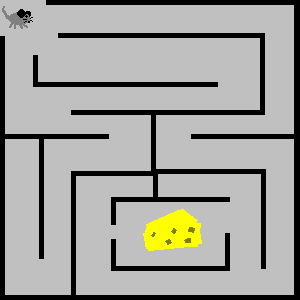
\includegraphics[width=\textwidth]{./media/mazeCheese}
    \end{column}

    \begin{column}{.5\textwidth}
    \begin{itemize}
        \item Simple model: \\ \hilite{``Mice love cheese''}.
        \bspace
        \item Put a mouse and some cheese together in a maze.
        \bspace
        \item How should the mouse get as much cheese as possible?
        \bspace
        \pause
        \item Do \hilite{not} provide a map.
    \end{itemize}
    \end{column}
  \end{columns}
\end{frame}

% Slide
\begin{frame}
\frametitle{A mouse in a maze}
\begin{itemize}
    \item The mouse faces a sequential decision problem.
    \bspace
    \item At each timestep $t$ the mouse must choose an \hilite{action}: \\
        \hspace{3mm} $a_t \in $ \{move up, down, left, right, eat\}.
    \bspace
    \item This choice of action will influence both: \\
        \hspace{3mm} its immediate \hilite{reward} $r_t$ (how much cheese it ate) \\
        \hspace{3mm} its \hilite{state} at the following time step $s_{t+1}$.
    \bspace
    \item The mouse's goal is to maximize its cumulative rewards through time, not just the reward in any single timestep $t$.
    \bspace
    \item We can model this problem as a \hilite{\emph{Markov Decision Process}}.
\end{itemize}
\end{frame}

% Slide
\begin{frame}{Markov Decision Process}
\begin{itemize}
    \item An \hilite{agent} taking actions in an \hilite{enivronment} $M$ (the MDP).
    \bspace
    \item \hilite{State} $s_t$ encodes the relevant data on the environment.
    \bspace
    \item \hilite{Action} $a_t$ is chosen by the agent.
    \bspace
    \item The agent receives a \hilite{reward} $r_t \sim R^M(s_t, a_t)$.
    \bspace
    \item The state \hilite{transitions} according to $s_{t+1} \sim P^M(s_t,a_t)$.
\end{itemize}
\end{frame}

% Slide
\begin{frame}{Maze as an MDP}
\begin{itemize}
    \item \hilite{Agent} $\leftrightarrow$ Mouse.
    \bspace
    \item \hilite{Environment} $\leftrightarrow$ Maze + Cheese.
    \bspace
    \item \hilite{State} $\leftrightarrow$ Position of the mouse.
    \bspace
    \item \hilite{Reward} $\leftrightarrow$ 1 if mouse eats cheese, 0 otherwise.
    \bspace
    \item \hilite{Transition} $\leftrightarrow$ Movement blocked by walls.
\end{itemize}
\end{frame}


% Slide
\begin{frame}{MDP notation}
\begin{itemize}
    \item Finite horizon MDP $M = (\Sc, \Ac, R^M, P^M, \tau, \rho)$.
    \bspace
    \item \hilite{Policy} $\mu$ is a function mapping each state $s \in \Sc$ and $i = 1,\ldots,\tau$ to an action $a \in \Ac$.
    \bspace
    \item For each MDP $M$ and policy $\mu$, we define a \hilite{value function}:
$$V^{M}_{\mu, i}(s) := \Exp_{M,\mu}\left[ \sum_{j=i}^{\tau} \overline{R}^M(s_j,a_j) \Big| s_i = s \right].$$
    \item A policy $\mu$ is \hilite{optimal} for the MDP $M$ if $V^{M}_{\mu, i}(s) = \max_{\mu'} V^{M}_{\mu', i}(s)$ for all $s \in \Sc$ and $i=1,\ldots,\tau$.
    \bspace
    \item We write \hilite{$\mu^M$ as the optimal policy for $M$}.
\end{itemize}
\end{frame}

%----------------------------------------------------------------------------
%----------------------------------------------------------------------------
\section{Reinforcement learning}

% Slide
\begin{frame}
\begin{block}{\Huge{Reinforcement learning}}
\end{block}
\end{frame}


% Slide
\begin{frame}
\frametitle{Reinforcement learning}
\begin{itemize}
    \item Agent interacts with an MDP just as before.
    \bspace
    \item \hilite{BUT} the agent is uncertain over dynamics $R^M$ and $P^M$. \\
    \bspace
    \item The agent observes the outcomes of the states and actions it visits and so can learn about the MDP through time.
    \bspace
    \item Fundamental tradeoff: \pause \hilite{exploration versus exploitation}.
    \pause
    \bspace
    \item \emph{The mouse only learns about where it actually goes.}
\end{itemize}
\end{frame}

% Slide
\begin{frame}
\frametitle{Reinforcement learning}
\begin{itemize}
    \item Repeated episodes of length $\tau$, initial distribution $\rho$. \\
        Episode $k$ starts at $t_k := (k-1) \tau + 1$.
    \bspace
    \item \hilite{RL algorithm} is a sequence $\{\pi_k \}_\Nat$ of functions mapping $H_{t_k}$ to a probability distribution $\pi_{k}(H_{t_k})$ over policies.
    \bspace
    \item We define the \hilite{regret} over episode $k$ wrt the MDP $M^*$:
        $$\Delta_k := \sum_{\Sc} \rho(s) (V^{M^*}_{\mu^*, 1}(s) - V^{M^{*}}_{\mu_k, 1}(s))$$
    \item And the regret to time $T$ of algorithm $\pi$:
        $${\rm Regret}(T, \pi, M^*) := \sum_{k=1}^{\lceil T/\tau \rceil} \Delta_k.$$
\end{itemize}
\end{frame}

% Slide
\begin{frame}
\frametitle{Why do we care?}
\begin{itemize}
    \item \st{Mice need to get more cheese!}
    \bspace
    \item MDPs are great models for sequential decision problems.
    \bspace
    \item \hilite{BUT} we rarely know the appropriate $R^M, P^M$ exactly.
    \bspace
    \item We want algorithms that will give us performance close to that of the unknown optimal controller for the unknown system!
    \bspace
    \pause
    \item Examples: \emph{healthcare, robotics, agriculture, finance and more.}
\end{itemize}
\end{frame}


% Slide
\begin{frame}
\frametitle{Algorithms for RL}

\begin{itemize}
	\item The \hilite{$\epsilon$-greedy} approach: \\
        \emph{Maintain estimate $\hat{M}$ for $M^*$. With probability $\epsilon$ choose a random policy otherwise use $\mu^{\hat{M}}$ certainty equivalent.}
    \bspace
    \item \hilite{Bayes-optimal} strategies: \\
        \emph{Mantain a posterior $\phi$ for $M^*$, choose $ \mu \in \arg \max_\mu \Exp [V^{M^*}_\mu]$.}
    \bspace
	\item \hilite{Optimism in the face of uncertainty}: \\
        \emph{Maintain a confidence set $\Mc_k$ that contains $M^*$ with high probability. Choose $\mu_k \in \arg\max_\mu \max_{M \in \Mc_k} V^{M_k}_{\mu}$.}
    \bspace
	\item \hilite{Posterior sampling}: \\
        \emph{Mantain a posterior $\phi$ for $M^*$. Every episode sample $M_k \sim \phi$ and choose $\mu^{M_k}$ which is optimal for that sample.}
\end{itemize}
\end{frame}

% Slide
\begin{frame}
\frametitle{Existing regret bounds}
\begin{itemize}
    \item Naive exploration ($\epsilon$-greedy, Boltzmann) generally take \hilite{exponentially} long in $|\Sc|, |\Ac|$ to learn the optimal policy.
    \bspace
    \item Bayes-optimal strategy usually computationally \hilite{intractable}.
    \bspace
    \item Optimism and posterior sampling are closely linked \cite{russo2013}.
    \bspace
    \item \hilite{State of the art} regret bounds \hilite{$\tilde{O}(|\Sc| \sqrt{|\Ac|T})$} attained by UCRL2 \cite{jaksch2010near} (optimism) and PSRL \cite{osband2013more} (sampling).
    \bspace
    \item Close to fundamental lower bounds $\Omega(\sqrt{|\Sc||\Ac|T})$.
\end{itemize}
\end{frame}

% Slide
\begin{frame}{Standard proof outline}
Write $V^*_{*,1}$ for $V^{M^*}_{\mu^{M^*}, 1}$ and similarly $k$ for $M_k$.
The episode regret:
$$\Delta_k = V^*_{*1} - V^*_{k,1}
= \left(V^*_{1}* - V^k_{k,1} \right) + \left(V^k_{k,1} - V^*_{k,1} \right) .$$
Using $M_k$ chosen optimistically, the first term is $\le 0$ with high probability.
For posterior sampling it is zero in expectation.
\bspace

The remaining term can be \hilite{decomposed into the Bellman error}:
\begin{equation*}
    \left(V^k_{k,1} - V^*_{k,1} \right) = \sum_{i=1}^\tau \left( \Tc^k_{k,i} - \Tc^*_{k,i} \right) V^k_{k,i+1} + \sum_{i=1}^\tau d_{t_k+i}.
\end{equation*}
where $d_i$ is a bounded martingale difference and $\Tc^M_\mu$ is the Bellman operator.
The contribution from bounded martingale differences is zero in expectation and bounded $O(\sqrt{T})$ with high probability.
\end{frame}

% Slide
\begin{frame}{Standard proof outline (cont.)}
The \hilite{Bellman operator} is defined
$$\mathcal{T}_{\mu}^{M} V(s) := \overline{R}^{M} (s, \mu(s)) + \sum_{s' \in \Sc} P^{M}(s' | s, \mu(s)) V(s').$$
Which, together with \hilite{H\"{o}lder's inequality} allows us to say:
\begin{equation*}
\label{eq: err sums}
    \sum_{i=1}^\tau \left( \Tc^k_{k,i} - \Tc^*_{k,i} \right) V^k_{k,i+1} \le
        \sum_{i=1}^\tau |\overline{R}^k - \overline{R}^* | + \frac{1}{2} \Psi_k \|P^k - P^* \|_1
\end{equation*}
Where $\Psi_k = max_{s,s'} V^k_{k,1}(s) - V^k_{k,1}(s')$ is the MDP span of $M_k$.
Standard \hilite{concentration inequalities} \cite{weissman2003inequalities} give the convergence of $R_k \rightarrow R^*$ and $P_k \rightarrow P^*$ at rate $\sqrt{\frac{1}{n}}$ and noting $\sum_{n=1}^T \sqrt{\frac{1}{T}} \le 2 \sqrt{T}$ completes the proof.
\end{frame}

% Slide
\begin{frame}{Problems with these bounds}
\begin{itemize}
    \item These bounds require $T = \Omega(|\Sc|^2 |\Ac|)$ for guarantees.
    \bspace
    \item \hilite{But} many problems have \hilite{$|\Sc|$ and $|\Ac|$ large or infinite!}
    \bspace
    \item Mouse in maze $|\Sc|=100, |\Ac|=5 \implies |\Sc|^2 |\Ac| = 50,000$.
    \bspace
    \item Factory line with 100 machines, each with 3 states, 3 actions: \\
        $|\Sc| = 3^{100}, |\Ac| = 3^{100} \implies |\Sc|^2 |\Ac| = 3^{300} \simeq 10^{150}$ \\
        Even lower bound $\sqrt{|\Sc||\Ac|T}$ requires $T =\Omega(|\Sc||\Ac|) \simeq10^{100}$
    \bspace
    \item How do you even deal with continuous $\Sc, \Ac$? \\
        \emph{Discretisation $\rightarrow$ \hilite{curse of dimensionality}.}

\end{itemize}
\end{frame}
%------------------------------------------------------------------------------
%------------------------------------------------------------------------------
% Factored MDPS
\section{Factored MDPs}

% Slide
\begin{frame}
\begin{block}{\Huge{Factored MDPs}}
\end{block}
\end{frame}

% Slide
\begin{frame}
\frametitle{A production line}
  \begin{columns}[T]
    \begin{column}{.5\textwidth}
        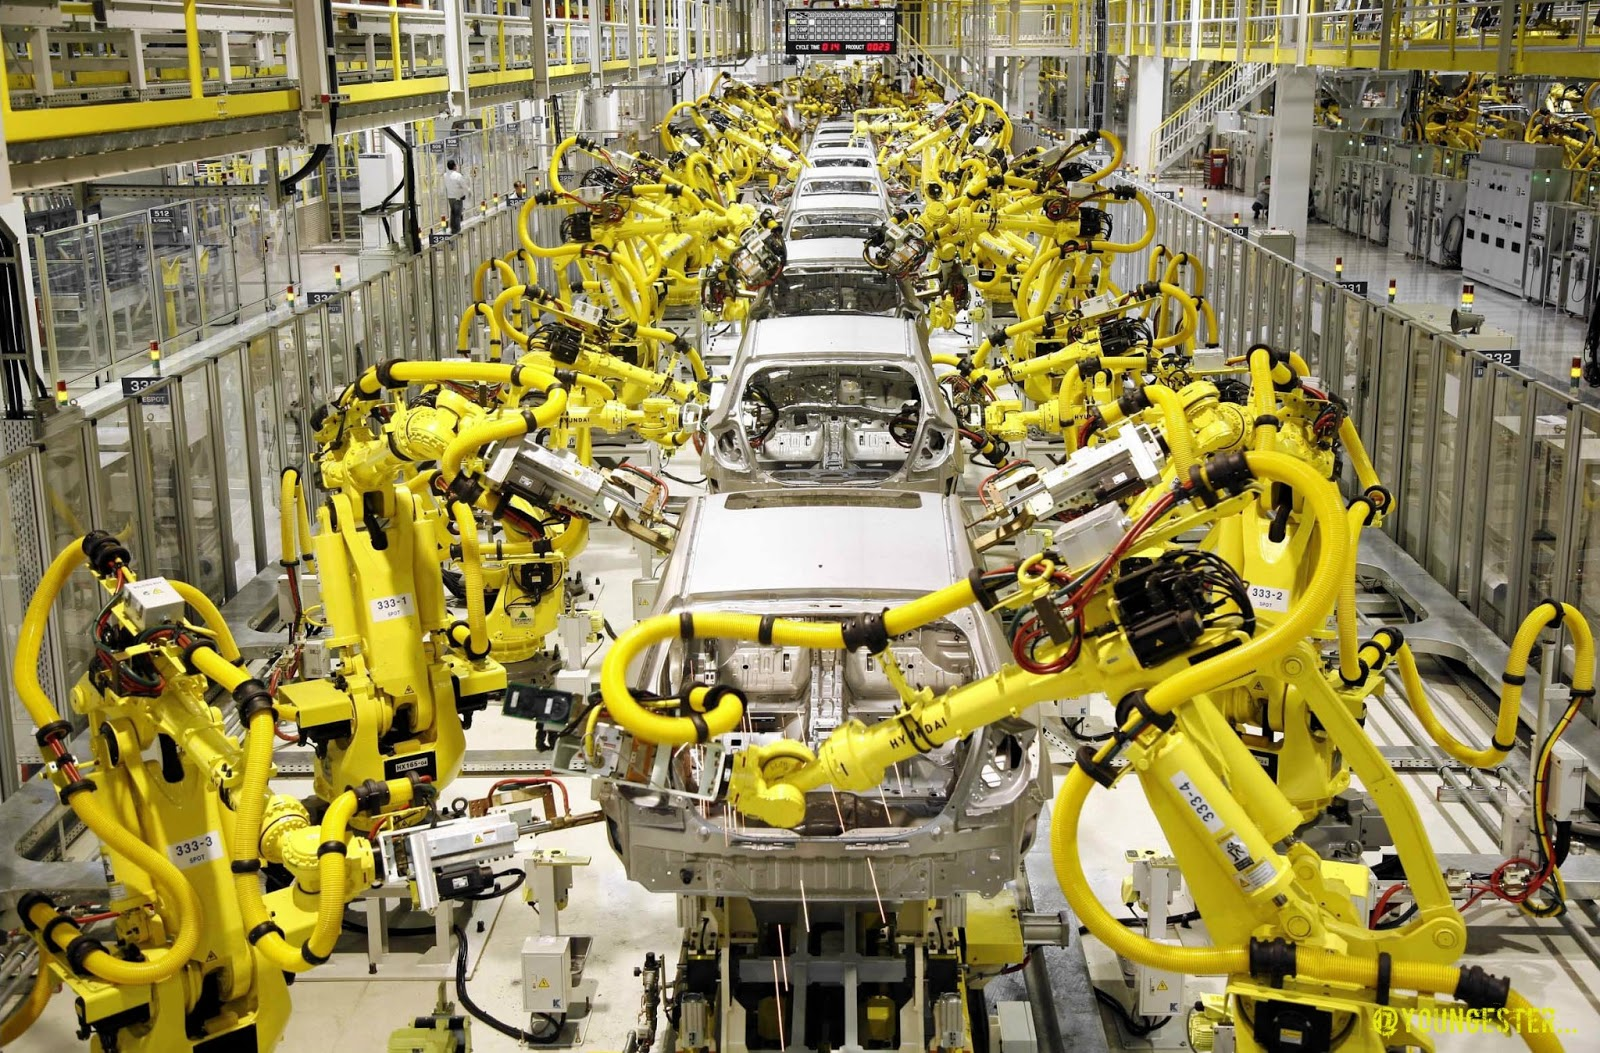
\includegraphics[width=\textwidth]{./media/productionLine}

        At each step, the rewards and transition of each machine only depend upon its neighbours.
    \end{column}

    \begin{column}{.5\textwidth}
    \begin{itemize}
        \item 100 \hilite{distinct} machines, each with 3 states and 3 actions.
        \bspace
        \item Each machine only \hilite{directly} affected by its neighbours.
        \bspace
        \item How should you operate the production line?
        \bspace
        \pause
        \item \hilite{Goal:} Exploit some low-dimensional structure.
    \end{itemize}
    \end{column}
  \end{columns}
\end{frame}

% Slide
\begin{frame}
\frametitle{Exploiting low-dimensional structure}
\begin{itemize}
    \item We know that over all MDPs regret $\Omega(\sqrt{|\Sc||\Ac|T})$.
    \bspace
    \item However, if we know that $M$ has some \hilite{low-dimensional structure} we can exploit this to improve guarantees.
    \bspace
    \item Previous works \cite{kearns1999efficient} showed loose sample complexity bounds for RL on factored MDPs. We prove the first regret bounds which are close to optimal.
    \bspace
    \item We can exploit the graphical structure of a factored MDP to obtain regret bounds that scale with the \hilite{parameters of the MDP}, which may be \hilite{exponentially smaller than $|\Sc|$ or $|\Ac|$}.
\end{itemize}
\end{frame}

% Slide
\begin{frame}
\frametitle{Factored MDPs}
Let $\Sc \times \Ac = \Xc = \Xc_1 \times .. \times \Xc_n$, $Z \subseteq [n]$ and
$ \Xc[Z] := \bigotimes\limits_{i \in Z} \Xc_i $

\begin{mydef}[ Factored transition functions $P \in \Pc \subseteq \Pc_{\Xc,\Sc}$ ]
$\Pc$ is factored over $\Xc = \Xc_1 \times .. \times \Xc_n$ and $\Sc = \Sc_1 \times .. \times \Sc_m$ with scopes  $Z_1, .. Z_m$ $\iff$,
for all $P \in \Pc, x \in \Xc, s \in \Sc$ there exist,
\begin{center}
$ P(s | x) = \prod_{i=1}^m P_i \left( s[i] \ \bigg\vert \ x[Z_i] \right) $
\hilite{$\leftarrow$ (conditional independence)}
\end{center}
\end{mydef}

\begin{mydef}[ Factored reward functions $R \in \Rc \subseteq \Pc^{C,\sigma}_{\Xc,\Real} $]
$\Rc$ is factored over $\Xc = \Xc_1 \times .. \times \Xc_n $ with scopes $Z_1, .. Z_l$ $\iff$, \\
for all $R \in \Rc, x \in \Xc$ there exist,
\begin{center}
$ \Exp [ R(x) ] = \sum_{i=1}^l \Exp\big[ R_i(x[Z_i]) \big] $
\end{center}
with \hilite{each $r_i \sim R_i(x[Z_i])$ and individually observed}.
\end{mydef}
\end{frame}


% Slide
\begin{frame}{Production line as a factored MDP}
\begin{itemize}
    \item \hilite{Agent} $\leftrightarrow$ Production manager.
    \bspace
    \item \hilite{Environment} $\leftrightarrow$ Production line and outputs.
    \bspace
    \item \hilite{State} $\leftrightarrow$ Machine states $s = (s_1, .., s_{100}) \in \{1, 2, 3\}^{100}$.
    \bspace
    \item \hilite{Reward} $\leftrightarrow$ Dollar output from each machine $r = \sum_{i=1}^{100} r_j$.
    \bspace
    \item \hilite{Transition} $\leftrightarrow$ Evolution of each machine state.
    \pause
    \item \hilite{Factored} since over one timestep $s_i$ only depends on its neighbours' states and actions $(s_k, a_k)$ for $k \in \{i-1, i, i+1\}$.
\end{itemize}
\end{frame}

%------------------------------------------------------------------------------
%------------------------------------------------------------------------------
% Main
\section{Main results}

% Slide
\begin{frame}
\begin{block}{\Huge{Main results}}
\end{block}
\end{frame}

% Slide
\begin{frame}
\frametitle{Main result}
% \begin{itemize}
    If the graph structure is known a priori, we can design algorithms which exploit this for \hilite{near-optimal regret bounds}.

    \bspace
    For example, in a factored MDP with $m$ distinct sections, each with $S$ states and $A$ actions we improve the regret bounds:

    \hilite{$$ \tilde{O} \left(\sqrt{(S^2 A)^m T} \right) \rightarrow
    \tilde{O} \left( m \sqrt{S^2 A T}\right) $$}

    Which is close to the optimal lower bound $\Omega(m \sqrt{SAT})$.

    \bspace
    \hilite{Key takeaway:} Regret polynomial in the \emph{parameters} encoding the factored MDP, which may be exponentially smaller than $|\Sc|$ or $|\Ac|$.
% \end{itemize}
\end{frame}

% Slide
\begin{frame}
\frametitle{Posterior Sampling for Reinforcement Learning}

\begin{algorithm}[H]
\label{alg: PSRL}

\begin{algorithmic}[1]
    \STATE \textbf{Input: }Prior $\phi$ encoding $\Gc$, $t=1$
    \FOR{episodes $k=1,2,..$}
        \STATE{sample $M_k \sim \phi(\cdot | H_{t})$}
        \STATE{compute near-optimal $\mu_k = \Gamma(M_k,\sqrt{\tau / k})$}  \textcolor{magenta}{$\leftarrow$(ADP planner)}

        \FOR{timesteps $j=1,..,\tau$}
            \STATE{sample and apply $a_t = \mu_k(s_t,j)$}
            \STATE{observe $r^1_t,..,r^l_t$ and $s^1_{t+1},..,s^m_{t+1}$}
            \STATE{$t = t+1$}
        \ENDFOR

    \ENDFOR
\end{algorithmic}
\end{algorithm}
\end{frame}

% Slide
\begin{frame}
\frametitle{UCRL-Factored}

\footnotesize
\begin{algorithm}[H]
\label{alg: UCRL-Factored}
\footnotesize
\begin{algorithmic}[1]
    \STATE \textbf{Input: }Graph structure $\Gc$, confidence $\delta$, $t=1$
    \FOR{episodes $k=1,2,..$}
        \STATE{$d_t^{R_i} = 4 \sigma^2 \log\left(4 l | \Xc[Z^R_i] | k / \delta\right)$ for $i=1,..,l$}
        \STATE{$d_t^{P_j} = 4 | \Sc_j | \log\left(4 m | \Xc[Z^P_j] | k  / \delta\right)$ for $j=1,..,m$}
        \STATE{ $\Mc_k = \{M \ | \Gc, \overline{R}_i \in \Rc^i_t(d_t^{R_i}), P_j \in \Pc^j_t(d_t^{P_j}) \ \forall i,j \}$} \textcolor{magenta}{$\leftarrow$(Confidence sets)}
        \STATE{compute near-optimistic $\mu_k = \tilde{\Gamma}(\Mc_k,\sqrt{\tau / k})$} \textcolor{magenta}{$\leftarrow$(Optim. ADP planner)}

        \FOR{timesteps $u=1,..,\tau$}
            \STATE{sample and apply $a_t = \mu_k(s_t,u)$}
            \STATE{observe $r^1_t,..,r^l_t$ and $s^1_{t+1},..,s^m_{t+1}$}
            \STATE{$t = t+1$}
        \ENDFOR

    \ENDFOR
\end{algorithmic}

\end{algorithm}
\end{frame}


% Slide
\begin{frame}
\frametitle{Main results}
\begin{theorem}[Expected regret for PSRL in factored MDPs]
\label{thm: reg PSRL}
If the prior $\phi$ is the distribution of $M^*$ and $\Psi$ is the span of the optimal value function:
\footnotesize
\begin{equation}
    \Exp \left[\mathrm{Regret}(T, \pi^{\rm PS}_{\tau}, M^*) \right] =
    \tilde{O}\left( \sigma \sum_{i=1}^{d_1} \sqrt{ | \Xc[Z^R_i] |T} + \Exp[ \Psi ] \sum_{j=1}^{d_2} \sqrt{|\Xc[Z^P_j]| |\Sc_j| T} \right)
\end{equation}
\end{theorem}


\begin{theorem}[High probability regret for UCRL-Factored]
\label{thm: reg UCRL-Factored}
If $D$ is the diameter of $M^*$, then for any $M^*$ can bound the regret of UCRL-Factored:
\footnotesize
\begin{equation}
    \mathrm{Regret}(T, \pi^{\rm UC}_{\tau}, M^*) =
    \tilde{O}\left( \sigma \sum_{i=1}^{d_1} \sqrt{ | \Xc[Z^R_i] |T} + C D \sum_{j=1}^{d_2} \sqrt{|\Xc[Z^P_j]| |\Sc_j| T} \right)
\end{equation}
\normalsize
with probability at least $1-\delta$
\end{theorem}
\end{frame}

% Slide
\begin{frame}
\frametitle{Discussion of results}

\begin{itemize}
    \item Close link between posterior sampling and optimism \cite{russo2013}.
    \bspace
    \item Bounds in expected regret versus high probability. Different MDP complexity measures, span $\Psi \le CD$ (diameter) $\le C \tau$.
    \bspace
    \item PSRL more \hilite{statistically and computationally} efficient \cite{osband2013more}.
    \bspace
    \item Known structure $\Gc$ \hilite{exponential $\rightarrow$ polynomial} regret.
    \bspace
    \item Both algorithms require approximate MDP planning.
    \bspace
    \item \hilite{Near optimal} as $m$ independent MDPs $\rightarrow$ $\tilde{O}(mS\sqrt{AT})$.

\end{itemize}
\end{frame}

% % Slide
% \begin{frame}
% \frametitle{Clean bounds in the symmetric case}
% Let $\Qc$ be shorthand for the structure $\Gc$ such that $l+1=m$, $C=\sigma=1$, $| \Sc_i | = |\Xc_i | = K$ and $|Z^R_i| = |Z^P_i | = \zeta$ for all suitable $i$ and write $J = K^\zeta$.
% In this case $\Psi, D \le \tau$ trivially.
% \vspace{2mm}

% \begin{corollary}[Clean bounds for PSRL]
% \label{cor: reg PSRL}
% \begin{equation}
%     \Exp \left[\mathrm{Regret}(T, \pi^{\rm PS}_{\tau}, M^*) \right]
%     \le 15m \tau \sqrt{J K T \log(2mJ T)}
% \end{equation}
% \end{corollary}

% \begin{corollary}[Clean bounds for UCRL-Factored]
% \label{cor: reg UCRL-Factored}
% \begin{equation}
%     \mathrm{Regret}(T, \pi^{\rm UC}_{\tau}, M^*) \le  15m \tau \sqrt{J K T \log(12mJT / \delta)}
% \end{equation}
% with probability at least $1-\delta$.
% \end{corollary}
% \end{frame}

% Slide
\begin{frame}{Bounds for the production line}
\begin{itemize}
    \item 100 different machines, each with 3 states and 3 actions.
    \bspace
    \item Transitions only depend on neighbours $\rightarrow$ \hilite{factored MDP}.
    \bspace
    \item $\Gc$-naive bounds $|\Sc| \sqrt{|\Ac|T} = 3^{250}\sqrt{T} \simeq 10^{120} \sqrt{T}$.
    \bspace
    \item Using $\Gc$ we obtain $ 100 \sqrt{(9)^3 3 T} \simeq 10^3 \sqrt{T}$.
    \bspace
    \item In general, \hilite{bounds exponentially tighter} than $\Gc$-naive.

\end{itemize}
\end{frame}



% Slide
\begin{frame}
\frametitle{Key lemma}
\begin{lemma}[Bounding factored deviations]
Let the transition function class $\Pc \subseteq \Pc_{\Xc,\Sc}$ be factored over $\Xc = \Xc_1 \times .. \times \Xc_n$ and $\Sc = \Sc_1 \times .. \times \Sc_m$ with scopes  $Z_1, .. Z_m$.
Then, for any $P,\tilde{P} \in \Pc$ we may bound their L1 distance:
$$ \| P(x) - \tilde{P}(x) \|_1 \le \sum_{i=1}^m \|P_i(x[Z_i]) - \tilde{P}_i(x[Z_i]) \|_1 $$
\end{lemma}
\hilite{Proof:}\\
We begin with the simple claim that for any $ \alpha_1, \alpha_2, \beta_1, \beta_2 \in (0,1]$:
\begin{eqnarray*}
    | \alpha_1 \alpha_2 - \beta_1 \beta_2 | &=& \alpha_2 \left| \alpha_1 - \frac{\beta_1 \beta_2}{\alpha_2} \right| \\
    &\le& \alpha_2 \left( \left|\alpha_1 - \beta_1 \right| + \left|\beta_1 - \frac{\beta_1 \beta_2}{\alpha_2} \right| \right) \\
    %&\le& \alpha_2 \left| \alpha_1 - \beta_1 \right| + \alpha_2 \frac{\beta_1}{\alpha_2} \left| \frac{\beta_1 \alpha_2}{\beta_1} - \beta_2 \right| \\
    &\le& \alpha_2 \left| \alpha_1 - \beta_1 \right| + \beta_1 \left| \alpha_2 - \beta_2 \right|
\end{eqnarray*}
\end{frame}


% Slide
\begin{frame}
\frametitle{Key lemma continued}
We now consider the probability distributions $p, \tilde{p} $ over $\{1,..,d_1\}$ and $q,\tilde{q} $ over $\{1,..,d_2\}$.
We let $Q = p q^T, \tilde{Q} = \tilde{p} \tilde{q}^T$ be the joint probability distribution over $\{1,..,d_1\} \times \{1,..,d_2\}$.
Using the claim above we bound the L1 deviation $\| Q - \tilde{Q} \|_1$ by the deviations of their factors:
\begin{eqnarray*}
    \| Q - \tilde{Q} \|_1 %&=& \sum_{i=1}^{d_1} \sum_{j=1}^{d_2} | Q_{i,j} - \tilde{Q}_{i,j} | \\
    &=& \sum_{i=1}^{d_1} \sum_{j=1}^{d_2} | p_i q_j - \tilde{p}_i \tilde{q}_j | \\
    &\le& \sum_{i=1}^{d_1} \sum_{j=1}^{d_2} q_j | p_i - \tilde{p}_i | + \tilde{p}_i | q_j - \tilde{q}_j | \\
    %&=& \sum_{i=1}^{d_1} |p_i - \tilde{p}_i | + \sum_{j=1}^{d_2} |q_j - \tilde{q}_j | \\
    &=& \| p - \tilde{p} \|_1 + \|q - \tilde{q} \|_1
\end{eqnarray*}
% Applying this result $m$ times to the factored transition functions $P$ and $\tilde{P}$ we recover our desired result.
We conclude the proof by applying this $m$ times to the factored transitions $P$ and $\tilde{P}$.
\end{frame}


% Slide
\begin{frame}
\frametitle{Conclusions}
\begin{itemize}
    \item \hilite{Regret polynomial in the parameters} encoding the factored MDP, which may be \hilite{exponentially smaller than $|\Sc|$ or $|\Ac|$}.
    \bspace
    \item Near-optimal regret bounds and simple algorithms.
    \bspace
    \item Two algorithms based on \hilite{posterior sampling} and \hilite{optimism}.
    \bspace
    \pause
    \item \hilite{BUT}:
    \begin{itemize}
        \item Algorithms require access to approximate MDP planner.
        \item You need to know $\Gc$ structure a priori.
        \item How can you learn without episodic reset $\tau$?
        \item What about other large/continuous MDPs with different structure, for example linear-quadratic control? \cite{osband2014model}.
    \end{itemize}
\end{itemize}
\end{frame}


% Slide
\begin{frame}
\frametitle{References}
\tiny{
\bibliography{referenceInformation.bib}
\bibliographystyle{unsrt}
}
\end{frame}

% Slide
\begin{frame}
\frametitle{Paper information}
\hilite{Near-optimal Reinforcement Learning in Factored MDPs}

Spotlight presentation at NIPS 2014

\bspace \bspace
Full paper is available at \textcolor{blue}{\url{http://arxiv.org/abs/1403.3741}}

\bspace \bspace
Author website \textcolor{blue}{\url{http://web.stanford.edu/~iosband/}}

\bspace \bspace
\hilite{Thanks for listening!}
\end{frame}
\end{document}
